\documentclass{article}

\usepackage{format}
\usepackage[utf8]{inputenc} % allow utf-8 input
\usepackage[T1]{fontenc}    % use 8-bit T1 fonts
%\usepackage{hyperref}       % hyperlinks
\usepackage[colorlinks=true, allcolors=blue]{hyperref} 
\usepackage{url}            % simple URL typesetting
\usepackage{booktabs}       % professional-quality tables
\usepackage{amsmath}
\usepackage{amsfonts}       % blackboard math symbols
\usepackage{nicefrac}       % compact symbols for 1/2, etc.
\usepackage{microtype}      % microtypography
\usepackage{graphicx}
\title{Investigating Token Ordering Strategies in Masked
Diffusion Models}

\author{
    Paul Bouchaud
    \And
    Arthur Djevahirdjian
}

\begin{document}
\maketitle

\begin{abstract}
In this project we benchmark masked diffusion models trained for Sudoku using different strategies to unmask tokens during inference, some from \citet{kim2025trainworstplanbest} plus another one based on entropy. We get results that do not always align with the original paper, but that still confirm the main hypothesis, which is that choosing a good order leads to much better performance.

\end{abstract}

\section{Introduction and motivation}
In the search of the best way to generate discrete data, two families of models have emerged:\\
autoregressive models and discrete diffusion models.

Autoregressive models (ARM) work by generating tokens from left to right according to a distribution
that gets learned in the training phase and depends on what has already been generated (plus a potential input).

From now on, we view ungenerated tokens as "masked", and thus focus on masked diffusion models, which are the most common
framework.

Masked (discrete) diffusion models (MDM) learn to unmask tokens by first learning
how to mask them following a differential equation (forward process) and then training to reverse the process.

This means that diffusion models can and are trained for unmasking tokens in any order, not just from left to right.
This means their training is much harder (\citet{kim2025trainworstplanbest}), and it is reasonable to say that if one does not take advantage of this more complex training on all orders, they might as well use ARMs, which are much easier to train. %Maybe add sources here

The paper \citet{kim2025trainworstplanbest} we study describes and tests several unmasking methods and concludes that they can lead to better accuracy than ARMs in the case of filling sudoku grids.

Our contribution is to test these strategies to see if the results line up, and we also compare them to another
unmasking method based on negative entropy.

Because the models we use have fewer parameters than the ones in \citet{kim2025trainworstplanbest} (1.3M vs 6M),
it will also give some clues on how the results scale with the size of the model.

The code we made for this experiment can be found in this repository:\\
\url{https://github.com/Brixfoly/GM-project}

\section{Background and research questions}
The big question is: 
to what extent does the bigger training overhead of MDMs
translate into them yielding better results, and for which types of data is it worth it compared to an autoregressive model ?

\subsection{Masked diffusion and adaptive decoding}
In the normal setting for MDMs, the neural net $\theta$ learns the reverse conditional distribution $p_\theta(.|x_t)$ (we assume that $t$ can be deduced from $x_t$ so we do not include it) which gives the probability to unmask tokens at any time.

After that, the most obvious way to generate data is at each step, choose some positions to unmask and unmask them according to $p_\theta$. Choosing the positions to unmask can be done in many ways, and we will see that it greatly affects performance.

The first way to do this is to choose a set of positions from a distribution that depends on parameters $(\alpha_t)$ that are linked to the diffusion differential equation. This is called `vanilla inference'.

Another way proposed by \citet{kim2025trainworstplanbest} is to choose according to a function $\mathcal{F}_\theta$ that gives a set of positions to unmask from a sequence of partially masked tokens. $\mathcal{F}_\theta$ is called an \textbf{inference strategy} and mostly depends on $p_\theta$.

If we think of denoising as solving a sudoku, this means that we strategically choose, given what we learned from $p_\theta$ which
move to make first when trying to fill a grid.
This is called `adaptive inference'.

\subsection{Main ideas of the reference paper}
\citet{kim2025trainworstplanbest} shows that, in the case of solving logical puzzle-like games,
\begin{itemize}
    \item Training an MDM to denoise using any path can be computationally unfeasible
    \item as a result, some inference paths are much harder to sample from than others
    \item adaptive inference with the right inference strategy can avoid these hard inference paths, and thus provide better performance
    \item the top-margin strategy is better than top-probability which is itself better than vanilla inference.
\end{itemize}

\subsection{Research hypotheses}
The paper assumes the 1RSB cavity prediction conjecture to prove the first point.
We will focus on the problem of filling a grid of sudoku.
Given that, we want to provide empirical evidence that supports the following hypothesis:
\begin{itemize}
    \item Adaptive inference that gives a score for each position and chooses the highest $K$ scores can be better than vanilla inference
    \item the top-margin inference strategy is better than top-probability
    \item using negative entropy as a score function can yield better results.
\end{itemize}

\section{Methodology}
\label{sec:methodology}

We benchmark these inference strategies on pretrained models for filling
Sudoku grids. The model weights remain fixed, so we compare the strategies
without additional training.

\subsection{Sudoku representation and common decoding procedure}
We represent a Sudoku grid as a sequence of 81 tokens, read row by row.
Digits from one to nine represent filled cells, and zero represents an empty,
or masked, cell. Only the given clues are filled in the initial grid.

At each step, the model predicts a probability distribution over the nine
possible digits for each masked cell. We then choose which cells to unmask
using one of the strategies described below, and fill each selected cell
with its most likely digit. When several cells are selected, their digits
come from the same model pass. The next pass uses the updated grid.

The original clues and previously filled cells remain unchanged. This means
that the decoder cannot correct an earlier mistake, so choosing which cells
to fill first can affect the final result. Reference solutions are used only
to evaluate the completed grids and are never given to the decoder.

\subsection{Token ordering strategies}
Let $x_t$ denote the current board at decoding time $t$, and let $M_t$ be the
set of its blank-cell indices. For a cell index $i\in M_t$ and a candidate
digit $j\in\{1,\ldots,9\}$, let $p_i(j)=p_\theta(x_i=j\mid x_t)$ denote
the model's predicted probability that cell $i$ contains digit $j$.
Let $p_i^{(1)}$ and $p_i^{(2)}$ be the largest and second-largest probabilities.
For each masked cell $i\in M_t$, the noise-free scores are
\begin{align*}
    s_{\mathrm{prob}}(i) &= p_i^{(1)}, \\
    s_{\mathrm{margin}}(i) &= p_i^{(1)}-p_i^{(2)}, \\
    s_{\mathrm{entropy}}(i) &= \sum_{j=1}^{9}p_i(j)\log p_i(j).
\end{align*}
Higher scores give higher priority. The entropy score is negative entropy,
so it prioritizes positions with lower predictive entropy.
Random ordering assigns independent uniform random scores to masked cells.

\subsection{Reveal budgets and ordering noise}
The number of cells to unmask at each step is randomly chosen following a
binomial distribution. With $T=50$ scheduled steps, let $m_r$ be the number
of cells still masked before step $r$, where $r=0,\ldots,T-1$. We choose
\[
    K_r\sim\mathrm{Binomial}\left(m_r,\frac{1}{T-r}\right).
\]
We then unmask the $K_r$ cells with the highest scores. The final step has
reveal probability one, so all remaining cells are filled. Decoding stops
early if every grid in the batch is already complete. A model pass predicts
distributions for the current batch; it can therefore reveal several cells
per grid rather than just one.

For a given seed and batch, we generate the reveal counts in advance and
reuse them for every strategy. This means that the strategies fill the same
number of cells at each step and differ only in which cells they choose.

We also test how adding noise to the ordering scores affects performance.
The reported checkpoint comparison uses no ordering noise. In a separate
experiment on the main DiT model, we compare no noise with a constant
Gumbel noise coefficient of $0.5$. For each adaptive score, we use
\[
    \widetilde{s}(i)=s(i)+\lambda G_i,
    \qquad G_i=-\log(-\log U_i),
    \qquad U_i\sim\mathrm{Uniform}(0,1),
\]
where the draws are independent across positions and steps, and
$\lambda\in\{0,0.5\}$ remains constant throughout decoding. Noise changes
which cells are selected, but each selected cell still receives its most
likely digit. Random ordering is not given additional noise.

These results use the implementation's \texttt{legacy-raw} convention,
which adds noise directly to the scores defined above. Since these scores
have different ranges, the same coefficient does not necessarily perturb
each strategy equally. The code also provides an \texttt{upstream} mode,
which uses maximum log-probability for probability ordering and decreases
the noise coefficient over time. The reported noise experiment does not
use that mode.

\subsection{Relationship to the reference paper}
We aim to check whether these token ordering strategies compare with each
other in the same way as in \citet{kim2025trainworstplanbest}. We implement
random, top-probability and top-margin ordering, and add negative entropy
as another score for choosing which cells to fill.

Our main model has approximately 1.3 million parameters, compared with
6 million for the paper's Sudoku MDM. We also evaluate four smaller encoder
checkpoints. These models have different architectures and training
histories from the paper's model. We use a fixed subset of the released
standard Sudoku test data and do not evaluate the separate hard test set.

All our models use the same decoding procedure, with greedy digit selection
and no changes to previously filled cells. Matching the paper's number of
steps or noise coefficient alone does not make the samplers identical.
We therefore treat this work as an independent comparison of ordering
strategies. If the results differ, model size, training and decoding choices
are all possible explanations; our experiments do not isolate their
individual effects.
\section{Experimental setup}
\label{sec:setup}

\subsection{Dataset and test instances}
For the experiments, we use 1,000 Sudoku puzzles taken from the 100,000-puzzle
 test set of the logic-puzzle repository~\citep{logicPuzzleData}. The puzzles
were sampled without replacement using reservoir sampling with seed 42. We
also save their original row IDs with the predictions, so we can always find
which puzzle a result corresponds to.

Each record contains the number of clues and then 81 cells, with their
coordinates, solution digits and strategy annotations. We use the coordinates
to rebuild the Sudoku grid, since the cells are not necessarily stored in grid
order. The model only sees the clues, with all empty cells represented by zero.
We reconstruct the full solutions separately and only use them to evaluate
the predictions.

The data loader checks that coordinates, digits, clue annotations and completed
solutions are valid. We also checked that the dataset checksum matches the
original release. We only use the standard test set here, not the separate
hard dataset used in the paper. We have not checked whether some of these
puzzles were also present in the pretrained models' training sets.

\subsection{Models and implementation}
Our main model is \texttt{tchauffi/sudoku-dit}, a pretrained diffusion
Transformer with 1,282,185 parameters~\citep{sudokuDiT}. To see whether the results depend on the model, we also test four checkpoints from \citet{sudokuEncoder}: \texttt{harry-100k},
\texttt{harry-500k}, \texttt{harry-combined} and \texttt{harry-hard}. They all
use the same Transformer encoder architecture with 806,154 parameters. 


We use the same decoding procedure for all models. At each step, the model
predicts the digits, we choose which empty cells to reveal, and then repeat.
The encoder checkpoints needed a small adaptation to work with this procedure.
They use token 10 for empty cells instead of zero, so we convert the input
before inference. We also remove the output score for digit zero and apply
softmax to the scores for digits 1 to 9. Another difference is that the DiT
receives the current decoding timestep in addition to the board, while the
encoders only receive the board. Because of this, our comparison is between
ordering strategies in a common decoder, not between the original sampling
procedures of the different repositories. Also, the checkpoint names alone
do not tell us exactly how each encoder was trained. We therefore cannot
explain differences between checkpoints only by their training data.

\paragraph{Original implementation and reused components.}
We implemented the dataset reconstruction, the four ordering methods, the
decoding loop and the evaluation code. The experiments can be resumed, and we
also implemented the paired comparisons. We reuse the published dataset and
pretrained weights. The DiT architecture is loaded using \texttt{nonet}, while
the encoder architecture was reproduced from its repository
~\citep{sudokuDiT,sudokuEncoder}. The decoder never changes clues or cells
that were already filled. We tested this behavior, as well as the reveal
counts, reproducibility, token conversion and checks for incompatible saved
results.

\subsection{Evaluation protocol and metrics}
For each checkpoint and ordering method, we run three experiments with seeds
0, 1 and 2. We use batches of 32 puzzles and a maximum of 50 decoding steps.
At every step, the number of cells to reveal is sampled from a binomial
distribution. For the same batch and seed, all ordering methods reveal the
same number of cells. This way, we compare which cells they choose, rather
than how many cells they reveal. For each chosen cell, we take the digit with
the highest predicted probability. Any remaining empty cells are filled at
the final step. If all puzzles are already complete, we stop earlier.

We first compare the checkpoints without adding noise to the ordering scores.
Then, in a separate experiment with the DiT, we compare noise coefficients
0 and 0.5. Here we use the \texttt{legacy-raw} setting: independent Gumbel
noise is added directly to each adaptive ordering score, with a fixed
coefficient at every step. This has no effect on random ordering. It is worth
noting that this is the older noise implementation, not the current
\texttt{upstream} default in our code. Between two conditions, we keep the
puzzles, their order, batch size, seeds, number of cells revealed and digit
prediction procedure unchanged.

The main metric is exact puzzle accuracy: a puzzle counts as correct only if
the entire predicted grid matches the reference solution. We also report the
percentage of predicted boards that respect the Sudoku constraints and keep
all the clues unchanged. Finally, we measure digit accuracy only on the
initially empty cells, without counting clues.

For inference cost, we record the average number of forward passes per puzzle
and the decoding time per batch. All experiments were run on CPU with
\texttt{PyTorch 2.15.0+cpu}, using four threads per process. The measured
decoding time does not include downloading the models, loading, warmup, data
transfers, evaluation or saving. Some checkpoint experiments ran in parallel
and shared CPU resources, so their timings are not a reliable way to compare
model speed.

We average the reported accuracies over the three seeds. For differences
between methods, we use a paired bootstrap over puzzles. First, we average
each puzzle's result across seeds. We then resample the 1,000 puzzles with
replacement 10,000 times and calculate the difference for each sample. Both
methods use exactly the same sampled puzzles. We use seed 20261105 for the
bootstrap and report the interval between the 2.5th and 97.5th percentiles.
These are descriptive 95\% intervals for the tested puzzles, models and seeds.
Even with three runs, we still have 1,000 different puzzles, not 3,000. We
also do not correct these intervals for multiple comparisons.

\section{Results and analysis}
\label{sec:results}

\subsection{Main comparison of ordering strategies}
The first result is that choosing cells based on the model predictions works
much better than choosing them randomly. Table~\ref{tab:main-results} shows
the results for the DiT without ordering noise, averaged over the three seeds.
Maximum probability solves 72.60\% of the 1,000 puzzles, while random ordering
only solves 0.70\%. This is an improvement of 71.90 percentage points, with
a paired 95\% bootstrap interval of $[69.73,74.07]$ percentage points. So,
for this setup, the results support H1.

\begin{table}[ht]
\centering
\caption{DiT results without ordering noise: 1,000 puzzles, seeds 0, 1 and 2,
and a 50-step binomial schedule with sampled digit values. Accuracy values
are percentages averaged over seeds; blank-cell accuracy excludes given clues.}
\label{tab:main-results}
\begin{tabular}{lrr}
\toprule
Method & Exact (\%) & Blank cells (\%) \\
\midrule
Random              & 0.70  & 51.06 \\
Maximum probability & 72.60 & 89.69 \\
Probability margin  & 71.57 & 89.38 \\
Lowest entropy      & 72.63 & 89.71 \\
\bottomrule
\end{tabular}
\end{table}

What is more interesting is that the three adaptive methods are close
in accuracy. Compared with maximum probability, margin gives
$-1.03$ percentage points, with a paired 95\% interval of $[-1.83,-0.23]$.
Entropy gives $+0.03$ percentage points, with an interval of
$[-0.83,0.90]$. These differences use the unrounded results, which explains
why they may not exactly match a subtraction of the values in
Table~\ref{tab:main-results}. The margin interval is below zero, suggesting
a small disadvantage compared with maximum probability in this experiment.
The entropy interval contains zero, so we do not see a clear advantage for
entropy over maximum probability. This does not mean that these two methods
are necessarily equivalent, only that our results do not show a clear
difference between them.

For every run in this comparison, Sudoku validity is equal to exact puzzle
accuracy. Looking at individual cells, the adaptive methods correctly predict
around 89--90\% of initially empty cells, compared with 51.06\% for random
ordering. This is much higher than exact puzzle accuracy because even one
wrong digit makes the whole puzzle incorrect. The average decoding time for
a run of 1,000 puzzles is between 34.49 and 36.87 seconds, although these
numbers should be interpreted carefully because the runs shared CPU
resources.

\subsection{Sensitivity to ordering noise}
The results change a lot when we add noise to the ordering scores. With the
DiT and a \texttt{legacy-raw} noise coefficient of 0.5, maximum-probability
accuracy goes from 72.60\% to 1.73\%. Margin goes from 71.57\% to 2.90\%,
and entropy from 72.63\% to 3.93\%. These are decreases of $70.87$, $68.67$
and $68.70$ percentage points, respectively. The results are shown in
Figure~\ref{fig:noise-results}.

\begin{figure}[ht]
\centering
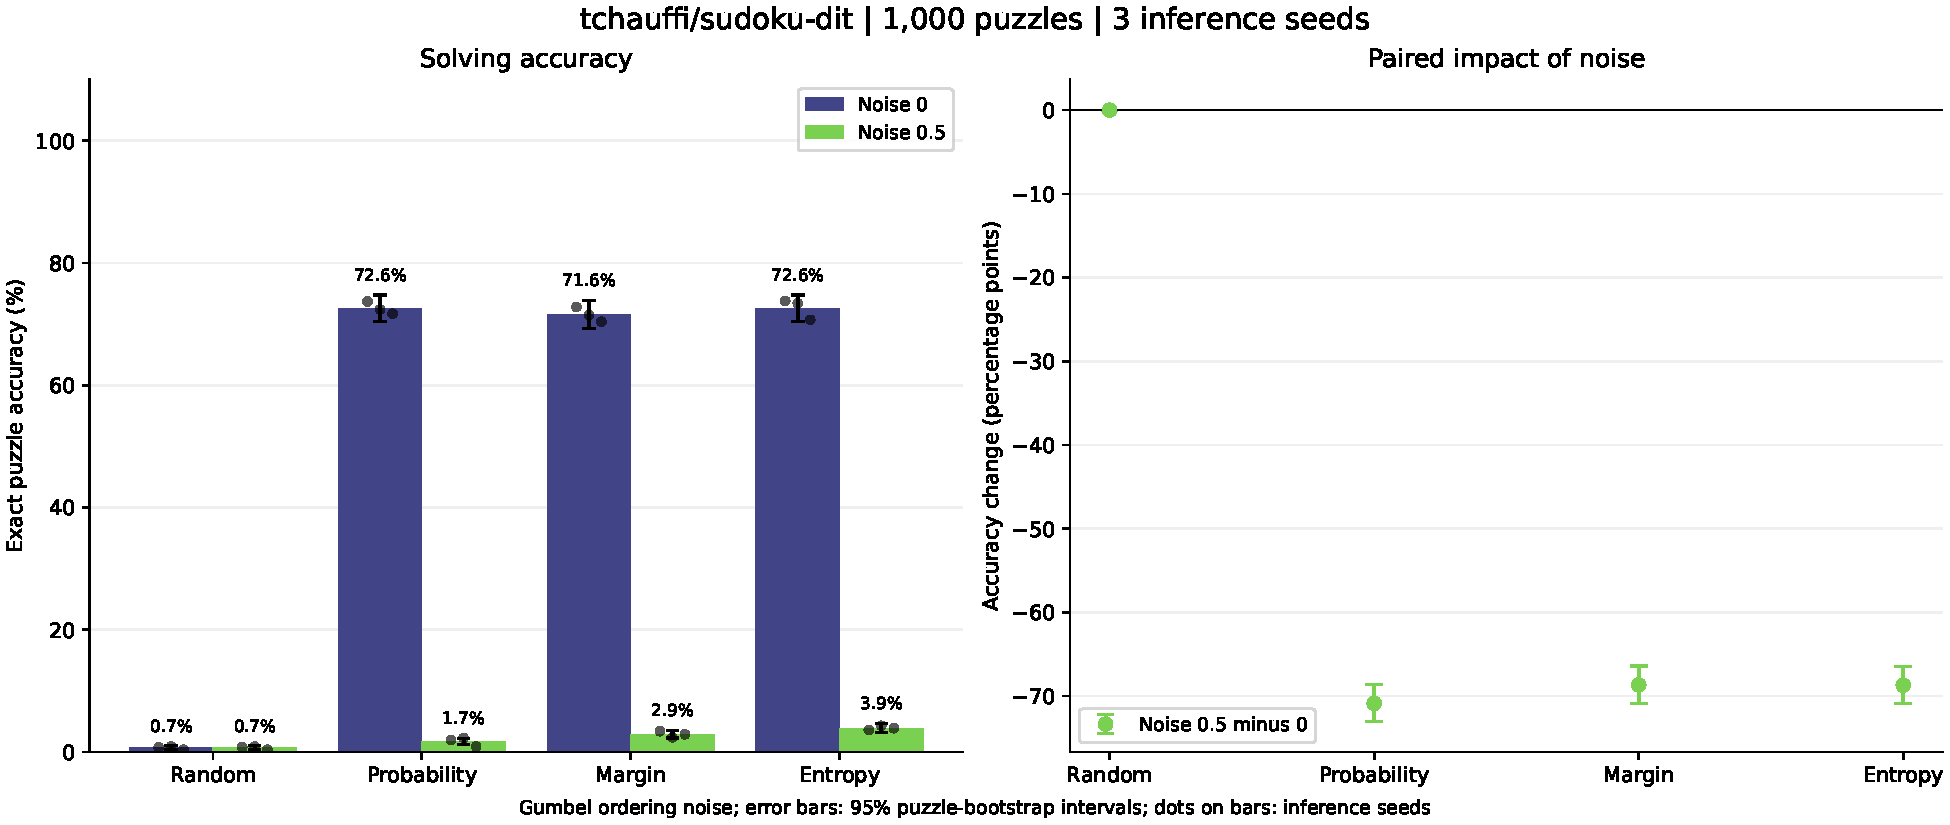
\includegraphics[width=\linewidth]{figures/noise_comparison.pdf}
\caption{Effect of constant raw-score Gumbel noise on the DiT, using the same
1,000 puzzles, three seeds and 50-step schedule with sampled digit values.
Bars show mean exact puzzle accuracy; black dots show individual seed
accuracies. The right panel shows changes from each method's zero-noise
result. Error bars are descriptive 95\% paired puzzle-bootstrap intervals.}
\label{fig:noise-results}
\end{figure}

As expected, random ordering stays at 0.70\%, and its predictions are
identical with and without noise. The inputs, reference solutions and number
of model passes are also the same in both conditions. The decrease in
accuracy therefore comes from the added ordering noise in this experiment.
However, the same coefficient does not have the same effect on all methods,
because probability, margin and entropy scores do not have the same scale.
These results show that the methods are very sensitive to this way of adding
noise. They do not tell us what would happen with the current
\texttt{upstream} noise implementation, or whether our results reproduce the
sampler used in the paper.

\subsection{Sensitivity to the model checkpoint}
We also wanted to check whether the improvement over random ordering depends
on the checkpoint. Table~\ref{tab:checkpoint-results} gives the results for
the four encoder checkpoints, together with the DiT results. Without noise,
all three adaptive strategies perform better than random ordering for every
checkpoint. For the encoders, the improvement of maximum probability over
random ordering ranges from 25.93 to 68.60 percentage points. All the
corresponding paired 95\% intervals are above zero. So the improvement in H1
is not limited to the DiT model.

\begin{table}[ht]
\centering
\caption{Exact puzzle accuracy (\%) without ordering noise, averaged over
three seeds on the same 1,000 puzzles and 50-step schedule with sampled
digit values. Sudoku validity rates equal exact accuracy in all 60
method--seed--checkpoint runs.}
\label{tab:checkpoint-results}
\begin{tabular}{lrrrr}
\toprule
Checkpoint & Random & Probability & Margin & Entropy \\
\midrule
\texttt{harry-100k}     & 0.07 & 26.00 & 25.13 & 25.70 \\
\texttt{harry-500k}     & 0.37 & 39.03 & 39.23 & 39.60 \\
\texttt{harry-combined} & 0.23 & 36.20 & 34.73 & 36.73 \\
\texttt{harry-hard}     & 0.60 & 69.20 & 69.43 & 69.67 \\
DiT                     & 0.70 & 72.60 & 71.57 & 72.63 \\
\bottomrule
\end{tabular}
\end{table}

There are also large differences between the encoder checkpoints themselves,
even though they have the same architecture. With maximum-probability
ordering, \texttt{harry-combined} performs 2.83 percentage points worse
than \texttt{harry-500k}, with an interval of $[-5.63,-0.03]$.
\texttt{harry-hard} improves on \texttt{harry-500k} by 30.17 percentage
points, with an interval of $[27.23,33.10]$. We can observe these differences,
but we cannot conclude that they come from the training data, since we did
not control the models' initialization, optimization or training history.

For the adaptive ordering methods, there is still no method that is clearly
best across all checkpoints. One exception worth mentioning is
\texttt{harry-combined}: margin is 1.47 percentage points below maximum
probability, with an interval of $[-2.60,-0.37]$. This difference between
margin and probability is itself 1.67 percentage points lower than for
\texttt{harry-500k}, with an interval of $[-3.10,-0.20]$. This may mean that
the effect of the ordering method depends on the checkpoint, but these are
exploratory comparisons and we have not corrected for multiple testing.
For the DiT, margin is also below maximum probability, by 1.03 percentage
points, with an interval of $[-1.83,-0.23]$. For the remaining checkpoints,
the margin-versus-probability intervals contain zero.
The entropy-versus-probability intervals also contain zero for every
checkpoint. We therefore cannot confirm the improvement expected in H3
from the zero-noise experiments.

\subsection{Scope of the hypothesis tests}
Overall, our experiments support H1: adaptive ordering is clearly better
than random ordering for the tested checkpoints, when no ordering noise is
added. However, they do not directly answer H2, which concerns ambiguous
predictions. To test that, we would need to identify ambiguous predictions
and compare the methods specifically on those cases. We also have not studied
confidence calibration or how accuracy changes with puzzle difficulty.
In particular, testing \texttt{harry-hard} on our standard test set is not
the same as testing on the separate hard dataset. Finally, similar average
accuracy does not mean that the methods make the same decisions or solve
exactly the same puzzles.

\section{Discussion and limitations}
\label{sec:discussion}

The first important result is that adaptive ordering works much
better than random ordering. This is true for all five checkpoints
we tested, even though their overall accuracies are quite
different. This confirms H1 in our experiments and shows that
the order in which the cells are filled has a major impact on
the final result.

However, the main difference with the original paper is the
comparison between maximum probability and probability margin.
We expected margin to perform better, but this is not what we
observe. For most checkpoints, both methods obtain almost the
same accuracy, and sometimes margin even performs slightly worse.
Lowest entropy also gives similar results. This does not mean
that the three methods are equivalent, but we cannot identify
a clear advantage for margin or entropy in our experiments.

One possible explanation is the size of the models. The DiT
we used has around 1.3 million parameters, while the model
used in the original paper is considerably larger. A smaller
model might produce different probability distributions,
making the distinction between maximum probability and margin
less useful. This could explain why we observe a large
difference between random and adaptive ordering, but almost
no difference between the adaptive methods themselves.
However, this is only a hypothesis. We would need to repeat
the experiments with larger models to determine whether
model size is actually responsible.

The Gumbel noise experiment also raises some questions.
With a coefficient of 0.5, maximum-probability accuracy drops
from 72.60\% to 1.73\%, with similar reductions for margin
and entropy. This is a very large decrease considering that
the model itself has not changed. Only the order in which
cells are selected is affected.

More importantly, it is not clear what the noise is supposed
to improve in this setting. The goal of the adaptive methods
is to select cells based on how confident the model is.
Adding noise to these scores can change that ordering and
make the selection less reliable. Noise could potentially
help introduce exploration or avoid repeatedly making
the same decisions, but we do not observe any benefit from
it in our experiments.

There is also some uncertainty about its implementation.
The original paper mentions adding Gumbel noise with a
coefficient of 0.5, without explaining precisely how this
noise is applied. We chose to add it directly to the ordering
scores, but other interpretations are possible. In addition,
the different ordering methods do not use scores on the same
scale, meaning that the same noise coefficient may affect
them differently. Our results therefore show the effect
of this particular implementation, rather than establishing
that Gumbel noise is generally harmful.


Our experiments also have some limitations. We evaluated
1,000 puzzles from the standard Sudoku test dataset using
three inference seeds. We did not test a separate hard
dataset or analyze the results according to puzzle difficulty.
We also use our own decoding procedure, which differs from
the original implementation in the paper, and we cannot
verify whether some test puzzles were present in the
models' training data.

For these reasons, our experiments are not an exact
reproduction of \citet{kim2025trainworstplanbest}. They still provide
a comparison of the ordering strategies under identical
decoding conditions, but the differences with the paper
cannot be attributed to a single factor.


\section{Conclusion and future work}
\label{sec:conclusion}

In this work, we compared four Sudoku cell-selection
strategies: random ordering, maximum probability,
probability margin and lowest entropy.

The main conclusion is that adaptive ordering clearly
improves accuracy compared with random ordering. However,
we were not able to reproduce the improvement of probability
margin over maximum probability reported in the original
paper. Instead, the three adaptive methods give very
similar results across most of our experiments.

We think the size and characteristics of the models could
be an important part of the explanation. In particular,
the smaller models used in our experiments might not
produce probability distributions for which margin provides
a real advantage over maximum probability. However,
our current experiments cannot confirm this explanation.

We also found that adding Gumbel noise with a coefficient
of 0.5 strongly reduces accuracy in our implementation.
This raises the question of whether this noise is actually
useful for Sudoku inference, and under which conditions
it could improve the results. Since the paper does not
fully describe how the noise is applied, further experiments
would be necessary before drawing conclusions about
the original method.

The most useful next step would be to repeat the comparison
with a larger model, ideally closer to the one used in
the paper. This would help determine whether model size
explains the missing improvement of probability margin.

It would also be interesting to analyze the probability
distributions produced by the models. In particular,
we could look at how often maximum probability and
margin select different cells, and whether these
differences affect the final solution. This would
allow us to investigate H2 more directly.

Finally, we would like to understand the role of Gumbel
noise more precisely. Comparing different ways of applying
the noise, and evaluating whether it actually improves
any ordering strategy, would help clarify whether it
is a useful part of the decoding procedure for bigger models.







\bibliographystyle{abbrvnat}
\bibliography{references_paper}




\end{document}
